\chapter{Swarm Intelligence Fundamentals}\label{cap:Swarm}
Swarm intelligence algorithms were inspired by several examples provided by nature. This inspiration was found on the behavior of social microorganisms, animals and insects, such as: ant colonies~\cite{ACO:Dorigo1999}\cite{ACO:Dorigo2005}\cite{ACS:Dorigo} \cite{MMAS:Kovarik}, fish schools \cite{FSS:Bastos-Filho2008}\cite{FSA:Yazdani2012}, bee colonies~\cite{ABC:Karaboga2005}\cite{BCO:Teodorovic2005}\cite{BCO:Teodorovic2006}\cite{BSO:Akbari2009}\cite{BSO:Akbari2010}\cite{BA:Pham2005}    \cite{BA:Pham2007}, flocks of birds~\cite{PSO:Eberhart1995}, swarms of fireflies~\cite{GSO:Krishnanand2009}\cite{FA:Yang2009}, bacterial colonies~\cite{BFO:Das2009}\cite{BFA:Muller2002}, among others.

The swarm intelligence algorithms are often applied to solve optimization problems without constraints. Some of these algorithms present good abilities do tackle some types of situations that may happen during optimization processes.

In the following sections, we describe some of the most used swarm intelligence algorithms for optimization and their variations to tackle continuous search spaces. Section \ref{sec:PSO} presents the Particle Swarm Optimization (PSO) algorithm. Section \ref{sec:APSO} describes the PSO algorithm with an adaptive behavior, called Adaptive Particle Swarm Optimization (APSO). Sections \ref{sec:ClanPSO} and \ref{sec:ClanAPSO} detail the PSO and APSO with communication topology based on clans, called Clan Particle Swarm Optimization (ClanPSO) and Clan Adaptive Particle Swarm Optimization (ClanAPSO), respectively. Section \ref{sec:ABC} presents the main concepts regarding Artificial Bee Colony (ABC). Finally, Section \ref{sec:FSS} presents the Fish School Search (FSS) algorithm.

\section{Particle Swarm Optimization - PSO}\label{sec:PSO}
Particle Swarm Optimization (PSO) is a computational intelligence technique proposed by James Kennedy and Russell Eberhart in 1995 \cite{PSO:Kennedy} \cite{PSO:Eberhart1995}\cite{PSO:Eberhart1995a} \cite{PSO:Schoene}. PSO is a population based algorithm inspired by the social behavior of flocks of birds that can be used to solve optimization and search problems. PSO was applied in many several real-world problems \cite{PSO:Wachowiak2004} \cite{PSO:Lu2002} \cite{PSO:Lian2006}.

In the PSO approach, the swarm is composed by a population of particles ($N$), where each particle $i$ has four attributes: the position within the search space $\vec x_i(t)$, that represents a possible solution for the problem; the velocity of the particle $\vec v_i(t)$, that is used to update the position of the particle $i$; the best position found by the particle during the search process $\vec p_i(t)$(also known as the cognitive memory); and the best position found by the neighborhood of the particle $\vec n_i(t)$ (also known as the social memory).

The neighborhood of the particle $i$ is the set of particles of the swarm from which the particle $i$ is able to acquire information. This information is used to update the swarm status (\textit{i.e.} velocity and position). The neighborhood is often defined by the communication topology. Different topologies were already proposed \cite{PSO:KennedyA}\cite{PSO:KennedyB} and the most used topologies are depicted in Figure~\ref{fig:topologies}.

\begin{figure}[!h]
\centering
\subfigure[]{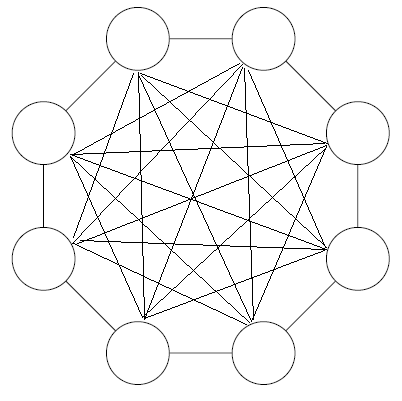
\includegraphics[scale=0.2]{image/Star.png}\label{fig:Star}}
\hspace{1mm}
\subfigure[]{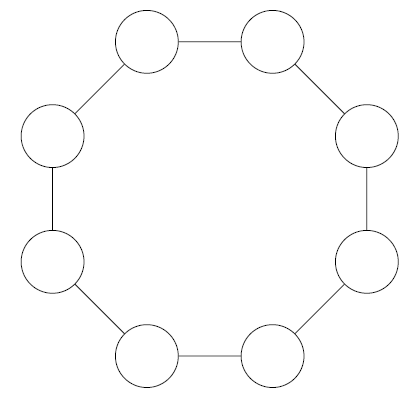
\includegraphics[scale=0.2]{image/Ring.png}\label{fig:Ring}}
\hspace{1mm}
\subfigure[]{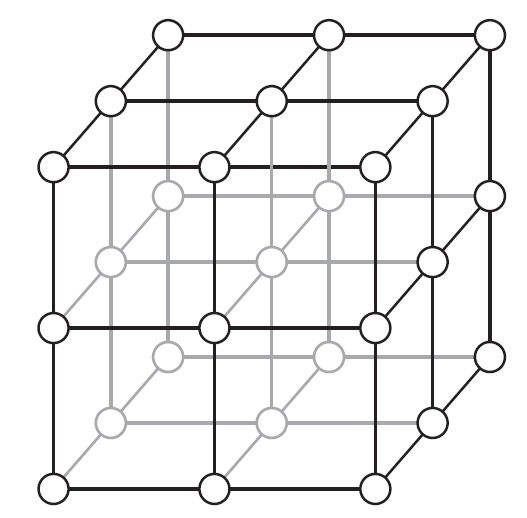
\includegraphics[scale=0.2]{image/vonneumann.png}\label{fig:vonneumann}}
\caption{Standard PSO communication topologies: (a) Star Topology used in $g_{best}$, (b) Ring Topology used in $l_{best}$ and (c) Von Neumann Topology.}
\label{fig:topologies}
\end{figure}

Figure \ref{fig:Star} presents the \emph{star} topology, in which the particles share information globally through a fully-connected structure. In this case, the information is quickly spread within the swarm and allows a quick convergence of the swarm. This topology is also known as global topology or $g_{best}$. Figure \ref{fig:Ring} presents the \emph{ring} topology, in which each particle is connected solely to $n$ neighbors. In this case, the information exchange mechanism allows a slower dissemination of information and helps to avoid local minima. The Ring topology is also known as local topology or $l_{best}$. The Von Neumann topology is depicted in Figure \ref{fig:vonneumann}. This is a balanced solution that consists in particles connected by a grid \cite{ClanPSO:Carvalho2009}.

The PSO execution occurs balancing the social learning and the individual learning of the individuals within the swarm. During each algorithm iteration, the particles move through the search space by updating their velocities and positions. There are several equations that can be used to update the velocity of the particles \cite{PSO:Clerc2002}. The most used equations to update the velocity and the position of particles are presented in the equations (\ref{eq:PSO_velocity}) and (\ref{eq:PSO_position}), respectively.
\begin{equation}\label{eq:PSO_velocity}
\vec v(t+1) = \omega \vec v(t) + r_1c_1[\vec p(t) - \vec x(t)] + r_2c_2[\vec n(t) - \vec x(t)],
\end{equation}

\begin{equation}\label{eq:PSO_position}
\vec x(t+1) = \vec x(t) + \vec v(t),
\end{equation}
in which $\vec v(t)$ is the velocity of particle in time step $t$, $r_1$ and $r_2$ are random numbers selected by using an uniform probability density distribution in the interval $[0,1]$. $c_1$ is the cognitive acceleration coefficient, $c_2$ is the social acceleration coefficient and $\omega$ is the inertial factor. $r_1c_1[\vec p(t) - \vec x(t)]$ is the cognitive component, which attracts the particle to its own best position ($\vec p(t)$), and $r_2c_2[\vec n(t) - \vec x(t)]$ is the social component, which attracts the particle to the best position found by its own neighborhood ($\vec n(t)$).

In the beginning of the algorithm execution, position ($\vec x(t)$) and velocity ($\vec v(t)$) of particles are attributed randomly. In the state-of-art \cite{PSO:Shi} \cite{PSO:Bratton2007}, the standard values of parameters $c_1$, $c_2$ are equal (2.05) and the inertial factor($\omega$) linearly decreasing from $\omega_{max} = 0.9$ to $\omega_{min} = 0.4$, along the iterations. Equation (\ref{eq:PSO_inertial}) calculates the linear decrement of the inertial factor \cite{PSO:Shi}.
\begin{equation}\label{eq:PSO_inertial}
\omega = \omega_{max} - \Bigl[(\omega_{max} - \omega_{min})\frac{g(t)}{g_{end}}\Bigr],
\end{equation}
where $g(t)$ is current iteration and $g_{end}$ is total number of iterations. The inertial factor optimizes the exploration-exploitation tradeoff. This decrement is done to allow the swarm to have a higher exploration ability in the initial iterations, and a higher exploitation capability in final iterations, when probably the swarm has found a good region of the search space to exploit.

\subsection{Pseudocode of the PSO Algorithm}
The pseudocode of the PSO algorithm is shown in Algorithm \ref{alg:PSO}. One can observe that the PSO algorithm, basically, consists on particle movement in search space (lines 6 and 7) and the update process of the cognitive (lines 9 and 10) and social memories (lines 12 and 13, respectively). The adaptation of inertial factor (line 16) allows the algorithm to regulate the exploitation-exploration tradeoff.

\begin{algorithm}[!h]
    Initialize particles of swarm\;
    Initialize inertial factor\;
    Initialize social and cognitive memory\;
    \While {the stop criterion is not achieved}{
        \For {each particle}{
            Update the velocity according to Equation (\ref{eq:PSO_velocity})\;
            Update the position according to Equation (\ref{eq:PSO_position})\;
            Evaluate the position using the objective function of problem\;
            \If{current position is better than cognitive memory}
            {
                Update the cognitive memory\;
            }
            \If{current position is better than social memory}
            {
                Update the social memory\;
            }
        }
        Update inertial factor according to Equation (\ref{eq:PSO_inertial})\;
    }
    \Return the social memory.
    \caption{Pseudocode of the PSO algorithm.}
    \label{alg:PSO}
\end{algorithm}

\section{Adaptive Particle Swarm Optimization - APSO}\label{sec:APSO}
Zhan \emph{et al.} proposed the Adaptive Particle Swarm Optimization (APSO) in 2009 \cite{APSO:Zhan2009}. This variation of PSO was proposed to solve two inefficiencies of the standard PSO algorithm: low convergence velocity and incapability to avoid local minima. The Adaptive PSO aims to achieve these goals with a systematic adaptation of the parameters and the use of an elitist learning strategy.

Basically, the APSO consists in a loop with the following steps: (\emph{i}) evaluate and estimate the distribution of particles in search space through the metric proposed by authors, called evolutionary factor; (\emph{ii}) classify the evolutionary state of the swarm; (\emph{iii}) determinate the acceleration coefficients based on the evolutionary state (improving the convergence velocity); (\emph{iv}) maintain the diversity with elitist learning strategy; and, (\emph{v}) adapt the inertial factor, increasing the efficiency of the search process.

\subsection{Estimation of Evolutionary Factor}
One needs to estimate the evolutionary factor in order to control the adaptation process of the APSO. To accomplish this, it is necessary to evaluate the distribution of the particles in the search space along the iterations. One needs to calculate the average Euclidian distance of each particle to the other particles of the swarm. The average distance ($d_i$) between particle $i$ and the rest of the swarm is evaluated by Equation (\ref{eq:APSO_distance}).
\begin{equation}\label{eq:APSO_distance}
d_i = \frac{1}{N-1}\sum_{j=1,j\neq i}^{N}\sqrt{\sum_{k=1}^{D}(x_i^k - x_j^k)},
\end{equation}
in which $N$ is the number of particles in the swarm and $D$ is the number of dimensions.

Then, the evolutionary factor ($f_{evol}$) is calculated according to Equation (\ref{eq:APSO_factor}).
\begin{equation}\label{eq:APSO_factor}
f_{evol} = \frac{d_g - d_{min}}{d_{max} - d_{min}} \ \  \in \ \ [0,1],
\end{equation}
in which $d_g$ is the average distance between the best particle of the swarm and the rest of the swarm, $d_{min}$ and $d_{max}$ are the smallest and the biggest average distance among all particles, respectively. To avoid $d_{min} = d_{max}$, it is necessary to have at least three particles in the population.

$f_{evol}$ is a number in the interval $[0,1]$. If the swarm is close to the best particle, then the evolutionary factor is close to $0$. On the other hand, if the particles of swarm are completely spread over the search space, then the evolutionary factor is close to $1$.

\subsection{Classification of Evolutionary State}
The original proposal of the APSO algorithm classifies the swarm in an evolutionary state using fuzzy rules. The evolutionary state is chosen at each iteration based on the membership function with higher value. Figure \ref{fig:factor_APSO} presents the four membership functions for the four evolutionary states: Convergence, Exploitation, Exploration and Jumping out.

\begin{figure}[!h]
\centering
 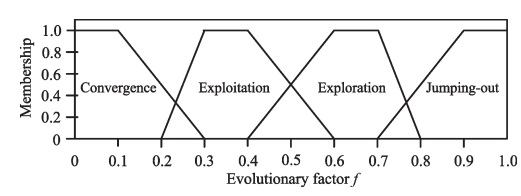
\includegraphics[width=0.65\textwidth]{image/factor}
 \caption{\small{Fuzzy membership functions for the APSO algorithm.}}
 \label{fig:factor_APSO}
\end{figure}

\emph{Convergence State}: it occurs when the value of the evolutionary factor is minimal and the particles are very close of the best particle. This means that the algorithm found a good region of the search space and then it is currently refining the solutions. We calculate the fuzzy value of this state according to Equation (\ref{eq:s_convergence}).
\begin{equation}
S_{convergence}(f_{evol}) = \begin{cases}
1,                 & \mbox{if $0.0 \leq f_{evol} \leq 0.1$}, \\
-5f_{evol} + 1.5,  & \mbox{if $0.1    < f_{evol} \leq 0.3$}, \\
0,                 & \mbox{if $0.3    < f_{evol} \leq 1.0$}.
\end{cases}
\label{eq:s_convergence}
\end{equation}

\emph{Exploitation State}: it occurs when the value of the evolutionary factor is shrunk and the particles are near to the best particle, it indicates that the swarm found a good region of the search space. The membership function of this state is defined according to Equation (\ref{eq:s_exploitation}).
\begin{equation}
S_{exploitation}(f_{evol}) = \begin{cases}
0,                &\mbox{if $ 0.0 \leq f_{evol} \leq 0.2 $}, \\
10f_{evol} - 2,   &\mbox{if $ 0.2 <    f_{evol} \leq 0.3 $}, \\
1,                &\mbox{if $ 0.3 <    f_{evol} \leq 0.4 $}, \\
-5f_{evol} + 3,   &\mbox{if $ 0.4 <    f_{evol} \leq 0.6 $}, \\
0,                &\mbox{if $ 0.6 <    f_{evol} \leq 1.0 $}.
\end{cases}
\label{eq:s_exploitation}
\end{equation}

\emph{Exploration State}: it occurs when the value of the evolutionary factor is medium to large and the particles have a medium or large distant of the best particle. In this case, the algorithm is trying to find a good region of the search space. We calculate the fuzzy value of this state according to Equation (\ref{eq:s_exploration}).
\begin{equation}
S_{exploration}(f_{evol}) = \begin{cases}
0,                &\mbox{if $ 0.0 \leq f_{evol}  \leq 0.4 $}, \\
5f_{evol} - 2,    &\mbox{if $ 0.4   <  f_{evol}  \leq 0.6 $}, \\
1,                &\mbox{if $ 0.6   <  f_{evol}  \leq 0.7 $}, \\
-10f_{evol} + 8,  &\mbox{if $ 0.7   <  f_{evol}  \leq 0.8 $},  \\
0,                &\mbox{if $ 0.8   <  f_{evol}  \leq 1.0 $}.
\end{cases}
\label{eq:s_exploration}
\end{equation}

\emph{Jumping out State}: it occurs when the evolutionary factor presents large values. This means that the APSO is jumping out of a local optimum to a new region, in other words, the globally best particle is distinctively away from the cluster of the swarm. The membership function of this state is defined according to Equation (\ref{eq:s_jumpingout}).
\begin{equation}
S_{jumping_out}(f_{evol}) = \begin{cases}
0,                  &\mbox{if $ 0.0 \leq f_{evol} \leq 0.7 $}, \\
5f_{evol} - 3.5,    &\mbox{if $ 0.7    < f_{evol} \leq 0.9 $}, \\
1,                  &\mbox{if $ 0.9    < f_{evol} \leq 1.0 $}.
\end{cases}
\label{eq:s_jumpingout}
\end{equation}

\subsection{Adaptation of Acceleration Coefficients}
The next step is to update the acceleration coefficients $c_1$ and $c_2$, which are initialized with values equal to 2.0 and are updated according to the current value of $f_{evol}$. The rules to update the coefficients are depicted in Table \ref{tab:apso_strategies}.

\begin{table}[!ht]
\caption{Strategies for the control of acceleration coefficients $c_1$ and $c_2$.}
\centering
\begin{tabular}{c c c}
\hline
Evolutionary State  &   $c_{1}$               &  $c_{2}$ \\
\hline
Convergence    & Increase slightly     & Increase slightly \\
Exploitation   & Increase slightly     & Decrease slightly \\
Exploration    & Increase              & Decrease \\
Jumping out    & Decrease              & Increase  \\
\hline
\end{tabular}
\label{tab:apso_strategies}
\end{table}

In the \emph{Convergence} state, the $c_1$ value is slightly increased and the $c_2$ value slightly is increased. In this state, the swarm is located at a minima, and, hence, the influence of social coefficient should be prioritized to guide other particles to this region. Thus, the value of $c_2$ should be increased. On the other hand, the value of the cognitive coefficient should be decreased to guarantee the swarm to converge faster. The consequence of this strategy is a premature saturation of the cognitive and the social coefficients to their lower and upper bounds, respectively. Thus, the swarm will strongly be attracted by the current best region, causing premature convergence, which is unsuitable if the current best region is just a local optimum. To avoid this, both $c_1$ and $c_2$ are slightly increased.

In the \emph{Exploitation} state, the $c_1$ value is slightly increased and the $c_2$ value is slightly decreased. In the Exploitation state, each particle uses local information and the swarm form groups in potential local optimal regions, that were identified by the historical best position of each particle. Hence, $c_1$ is slowly increased and maintains a relatively large value to predominate the search and exploitation around the respective cognitive memories. Probably, the social memory is still not present in the global optimal region. Therefore, decreasing $c_2$ slowly can avoid the lock in local optimal. Furthermore, an exploitation state in more likely to occur after an exploration state and before a convergence state. Hence, changing directions for $c_1$ and $c_2$ should be slightly altered from the exploration state to the convergence state \cite{APSO:Zhan2009}.

In the \emph{Exploration} state, the $c_1$ value is increased and the $c_2$ value is decreased. In this state, is essential the swarm should explore so many optima search regions as possible. hence, increasing $c_1$ and decreasing $c_2$ can help each particle explores individually and achieve its own historical best positions. In this case, we aim to avoid that the current best particle of swarm get stucked in a local optimum.

In the \emph{Jumping out} state, the $c_1$ value is decreased and the $c_2$ value is increased. When the best particle is jumping out of the local optimum toward a better optimum, it is very likely to be far away from the core of the swarm in presented in the Convergence state. As soon as this new region is found by a particle, which becomes the (possibly new) guide, others should follow it and achieve this new region as fast as possible. To guarantee this behavior of the swarm, a large $c_2$ value together with a relatively small $c_1$ value is more indicated.

The incremented or decremented value of acceleration coefficients is called acceleration rate ($\delta$). In the APSO algorithm, this value is a random number uniformly generated  among the interval [0.05, 0.1]. The term ``slightly'' found in strategies of Convergence and Exploitation states, implies in the use of acceleration rate equal to 50\% ($\delta \cdot 0.5$).

In the coefficients adaptation process, they can achieve huge or small values, generating unstable moments in search process. To solve this, the authors of APSO proposed a normalization of acceleration coefficient values. The lower and upper boundaries of acceleration coefficients are $c_{min} = 1.5$ and $c_{max} = 2.5$, respectively. If the sum of $c_1$ and $c_2$ is larger than 4.0, the acceleration coefficients should be normalized according to Equation (\ref{eq:APSO_normalized}).
\begin{equation}\label{eq:APSO_normalized}
c_i = \frac{c_i(c_{min} + c_{max})}{c_1 + c_2}, \ \ i = 1,2.
\end{equation}

\subsection{Elitist Learning Strategy}
The third step is the application of a operator in order to generate diversity. The authors named it as Learning Strategy using Elitism and this mechanism aims to improve the global search capability of the algorithm. It was first proposed to be applied just in the best particle during the Convergence state, generating the Jumping out state.

The reason for this operator is because the best particle does not have exemplars to follow. As a means to improve its own, a perturbation was developed to help the best particle to push itself out of a local minima to a potential better search region. If the new region is better, then the rest of swarm will follow quickly the leader in order to converge to this new search region.

This is a type of greedy local search applied only in one dimension ($d$) of the current best particle ($\vec n_i (t)$) of the swarm aiming to allow this particle to escape from a local optimum. All the dimensions have the same probability to be chosen. The Gaussian mutation is generated according to Equation (\ref{eq:APSO_elitism}).
\begin{equation} \label{eq:APSO_elitism}
\vec n_i(t+1) = \vec n_i(t) + (X_{max}^d - X_{min}^d)G(\mu,\sigma^2),
\end{equation}
in which $(X_{max}^d, X_{min}^d)$ are the boundaries of search space, $G(\mu,\sigma^2)$ is a random number generated by Gaussian distribution with a zero mean $\mu$ and standard deviation $\sigma$, which is called the elitist learning rate. The authors suggested that $\sigma$ be linearly decreased with the iterations number and is calculated by Equation (\ref{eq:apso_sigma}).
\begin{equation} \label{eq:apso_sigma}
\sigma = \sigma_{max} - \Bigl[(\sigma_{max} - \sigma_{min})\frac{g(t)}{g_{final}}\Bigr],
\end{equation}
in which ($\sigma_{max},\sigma_{min}$) are the boundaries of $\sigma$, $g(t)$ is the current iterations and $g_{final}$ is the total number of iterations. In empirical tests, Zhan \emph{et al.} proposed to use $\sigma$ = 1.0 in the beginning of the simulations, with the objective to escape from a local optimum and decrease it to $\sigma$ = 0.1 at the end of the simulation, to refine the found solutions.

The position of the best particle is updated only if the new position found by the operator is better than the previous one. Otherwise, the new position will replace the worst particle in the swarm.

\subsection{Adaptation of Inertial Factor}
In the last step, the inertial factor $\omega$ is updated using equation (\ref{eq:APSO_inertial}) in order to auto-adapt the exploration-exploitation ability of the swarm.
\begin{equation}\label{eq:APSO_inertial}
\omega(f_{evol}) = \frac{1}{1 + 1.5e^{-2.6f_{evol}}} \ \ \in \ \ [0.4;0.9], \ \ \forall f_{evol} \ \ \in \ \ [0,1].
\end{equation}

\subsection{Pseudocode of the APSO Algorithm}
The pseudocode of the APSO algorithm is shown in Algorithm \ref{alg:APSO}. The APSO algorithm has the same main steps that are found in the PSO algorithm. However, one can observe the adaptation of parameters (acceleration coefficients and inertial factor) in the lines 3 to 20. In lines 3 to 6, one can observe the steps needed to estimate the evolutionary factor. The classification of evolutionary state of swarm can be observed in lines 7 and 8. In the lines 9 and 10, one can observe the adaptation of acceleration coefficients. In line 11, the adaptation of inertial factor is executed. In the lines 12 to 19, one can observe the execution of elitist learning strategy.

\begin{algorithm}[!h]
    Initialize particles of swarm\;
    \While {the stop criterion is not achieved}{
        \For {each particle}{
            Calculate the average distance according to Equation (\ref{eq:APSO_distance})\;
        }
        Calculate the evolutionary factor according to Equation (\ref{eq:APSO_factor})\;
        Calculate the membership function according to Equations (\ref{eq:s_convergence}), (\ref{eq:s_exploitation}), (\ref{eq:s_exploration}) and (\ref{eq:s_jumpingout})\;
        Classify the swarm in the evolutionary state\;
        Adapt the acceleration coefficients according to Table \ref{tab:apso_strategies}\;
        Normalize the acceleration coefficients according to Equation (\ref{eq:APSO_normalized})\;
        Update the inertial factor according to Equation (\ref{eq:APSO_inertial})\;
        \If{classified on \emph{Convergence} state}
        {
            Generate a new position using the Equations (\ref{eq:APSO_elitism}) and (\ref{eq:apso_sigma})\;
            \If{new position is better than the best cognitive memory}
            {
                Update the position and cognitive memory of the best particle\;
            }
            \Else
            {
                Update the position and cognitive memory of the worst particle\;
            }
        }
        \For {each particle}
        {
            Update the social memory in neighborhood\;
            Update the velocity according to Equation (\ref{eq:PSO_velocity})\;
            Update the position according to Equation (\ref{eq:PSO_position})\;
            Evaluate the position using the objective function of problem\;
            \If{current position is better than cognitive memory}
            {
                Update the cognitive memory\;
            }
            \If{current position is better than social memory}
            {
                Update the social memory\;
            }
        }
    }
    \Return the social memory.
    \caption{Pseudocode of the APSO algorithm.}
    \label{alg:APSO}
\end{algorithm}

\section{Clan Particle Swarm Optimization - ClanPSO}\label{sec:ClanPSO}
Clans are groups of individuals united by a kinship based on a lineage, for example. Some clans stipulate a common ancestor to become the leader of the clan, and every individual of the clan will be guided by this leader. Incorporating this characteristic, a topology was proposed for improving the PSO algorithm performance, the Clan Particle Swarm Optimization \cite{ClanPSO:Carvalho2008}. This topology consists in a set of clan, where each clan is sub-swarm and uses a fully-connected structure to share information. The structure presented in Figure \ref{fig:clans} is an example with four clans (A, B, C and D) of five particles.
\begin{figure}[!h]
\centering
 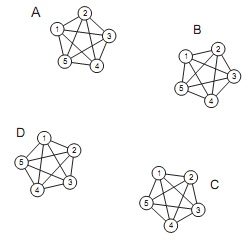
\includegraphics[width=0.35\textwidth]{image/Clan}
 \caption{\small{Example of division of the population in sub-swarms.}}
 \label{fig:clans}
\end{figure}

Other approach was proposed that enables the migration of particles among clans and some improvements were reached for some benchmark function \cite{ClanPSO:Carvalho2009}. However, there are some problems in this case, such as possibility of empty clans.

In this algorithm, the population size is divided according to the number of particle per clan ($N_{pc}$). For each iteration, each one of clans performs a search using a classical PSO and selects the particle that had achieved the best position of the entire clan. This particle is called the leader and this process of marking is called delegation. After the definition of all leaders, we form a new swarm with only the leaders of clans and we execute the PSO algorithm just with the leaders. This process is called conference of leaders. We can observe in more details these execution steps of the ClanPSO algorithm.

\subsection{Delegation of Leaders}
Is similarly to complex social behavior, with several clans with various leaders. The definition of a leader in clan is a marking process the best particle in the swarm, for example in Figure \ref{fig:leaders}. The delegation process is based in the global information exchange mechanism inside each clan, which uses $\vec{n_{best}}$ information to delegate the leader.
\begin{figure}[!h]
\centering
 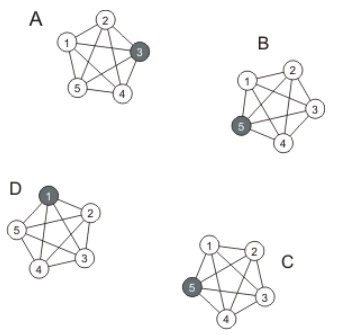
\includegraphics[width=0.35\textwidth]{image/Leaders}
 \caption{\small{Example of definition of clans leaders (A, B, C and D).}}
 \label{fig:leaders}
\end{figure}

\subsection{Conference of Leaders}
After the delegation, the leaders need to adjust their positions based on the best leader. This second step consists in execution of PSO only with the leaders, and is called conference of leaders. The conference can be performed using either the star (observe Figure \ref{fig:conference_star}) or ring (observe Figure \ref{fig:conference_ring}) topology.

\begin{figure}[!h]
\centering
\subfigure[]{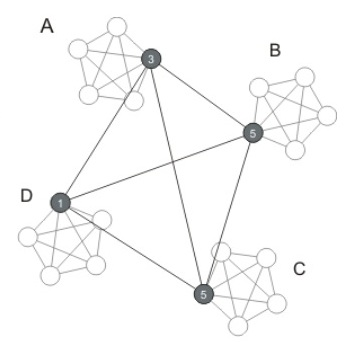
\includegraphics[scale=0.5]{image/conference_star}\label{fig:conference_star}}
\hspace{1mm}
\subfigure[]{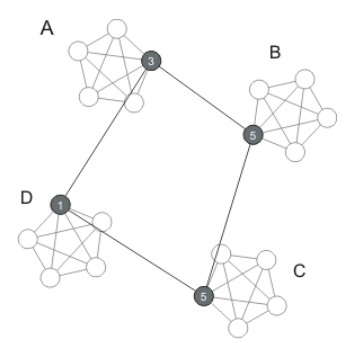
\includegraphics[scale=0.5]{image/conference_ring}\label{fig:conference_ring}}
\caption{Types of conference in the ClanPSO: (a) global conference and (b) local conference.}
\label{fig:conference}
\end{figure}

The topology to be used depends on the kind of problem to be solved. When the star topology is used, the information is spread faster between leaders through of global information share, guaranteeing a better exploitation ability. When is used ring topology, the communication between leaders is slower, thus the algorithm has great exploration ability. The convergence velocity is smaller than in star topology, but the quality of the solutions are often better.

\subsection{The Information shared within the clans}
After the leaders conference, the leaders will return to its respective clans and the new information acquired in the process will be widely used inside each clan to adjust the other particles. Indirectly, allows that all other particles be guided by the best position found within the entire topology. Through indirect communication, a foreign leader does not directly influence another clan, and then preserves the  exploration capacity of clans.

\subsection{Pseudocode of the ClanPSO Algorithm}
The pseudocode of the ClanPSO algorithm is shown in Algorithm \ref{alg:ClanPSO}. In the lines 4 to 14, one can observe the PSO execution within of each clan. In lines 17 to 28, one can observe the leaders conference. We can observe the leaders delegation in the lines 5 and 16, and still the line 5, the return of information from the leaders conference.

\begin{algorithm}[!h]
    Initialize the particles with random positions and velocities\;
    Group the particles in clans with global topology\;
    \While {the stop criterion is not achieved}{
        \For {each clan}{
            Find the best particle and mark as leader\;
            Update the velocity according to Equation (\ref{eq:PSO_velocity})\;
            Update the position according to Equation (\ref{eq:PSO_position})\;
            Evaluate the position using objective function of the problem\;
            \If{new position is better than cognitive memory}
            {
                Update cognitive memory\;
            }
            \If{new position is better than social memory}
            {
                Update social memory\;
            }
        }
        Add clan leader in the leaders list\;
        \For {each leader particle of the list}
        {
            Find the best particle\;
            Update the velocity according to Equation (\ref{eq:PSO_velocity})\;
            Update the position according to Equation (\ref{eq:PSO_position})\;
            Evaluate the position using objective function of the problem\;
            \If{new position is better}
            {
                Update cognitive memory\;
            }
            \If{new position is better than social memory}
            {
                Update social memory\;
            }
        }
    }
    \Return the social memory.
    \caption{Pseudocode of the ClanPSO algorithm.}
    \label{alg:ClanPSO}
\end{algorithm}

\section{Clan Adaptive Particle Swarm Optimization - ClanAPSO}\label{sec:ClanAPSO}
The Clan Adaptive Particle Swarm Optimization (ClanAPSO) was developed in 2011 \cite{ClanAPSO:Pontes2011}. This algorithm was proposed by aggregation of the process of systematic adaptation of parameters with a search strategy of multi-swarm. This technique was inspired in the clans topology presents in the ClanPSO algorithm combined to the concepts of parameters adaptation and elitist strategy found in the APSO algorithm.

The ClanAPSO algorithm presents an adaptation process in each swarm in a multi swarm system, this allows that sub-swarms can perform different types of search by iteration of the algorithm, \textit{i.e.} it is possible to perform exploitation and exploration search simultaneously in distinct regions of the search space. The concept of clans is interesting because it allows to identify local leaders of groups of particles (clans) and carry out the information share between clans indirectly. The indirect communication between clans promotes improvement the search process because it is a distributed process of spreading information.

There are two versions of the ClanAPSO algorithm. The original version \cite{ClanAPSO:Pontes2011} executes the APSO algorithm within the clans and also execute the APSO in the conference of leaders. The proposed second version \cite{ClanAPSO:Vitorino2011} also includes the adaptation capability within the clans, but in the leaders conference is running the PSO algorithm.

\subsection{Pseudocode of the ClanAPSO Algorithm}
The simplified pseudocode of the ClanAPSO algorithm is shown in Algorithm \ref{alg:ClanAPSO}. In the lines 3 to 6, the APSO execution within of each clan is presented. In the lines 7 and 8, one can observe the conference of leaders, where they can be executed by the APSO algorithm or the PSO algorithm. We can observe the leaders delegation in the line 5.

\begin{algorithm}[!h]
    Initialize the particles with random positions and velocities\;
    \While {the stop criterion is not achieved}{
        \For {each clan}{
            Execute APSO within the clans\;
            Delegate leader\;
        }
        Create conference of leaders\;
        Execute APSO (or PSO) with the leaders\;
    }
    \Return the best particle.
    \caption{Pseudocode of the ClanAPSO algorithm.}
    \label{alg:ClanAPSO}
\end{algorithm}

\section{Artificial Bee Colony - ABC}\label{sec:ABC}
The ABC algorithm was proposed by Karaboga in 2005 \cite{ABC:Karaboga2005}. ABC is an algorithm of search and optimization modeled by the behavior of honey bees \cite{ABC:Karaboga2006} \cite{ABC:Karaboga2007} \cite{ABC:Karaboga2009a} \cite{ABC:Karaboga2009b} \cite{ABC:Ziarati2011}. The bee colony is one of the natural societies with the most specialized social divisions. In the simplified model assumed by the ABC, the bee colony is composed by three types of bees: employed bees, onlookers and scouts. Initially, the swarm is divided in equal parts of employed bees and onlookers bees. The employed bees are those that go to the food source explored by herself, there is a food source to each employed bee. The bees that wait in the hive and decide to exploit a food source depending on the information shared by the employed bees are called onlooker bees. The onlookers are guided bees. When the food source does not improve its quality, the associated employed bee is now scout bee, which is responsible to find a new valuable food source. We will call them guide bees in exploration mode.

Basically, the steps of the algorithm executed in each iteration are: (\emph{i}) the employed bees explore its respective food sources; (\emph{ii}) it is determined the quality of food sources, which are shared to onlooker bees; (\emph{iii}) the onlooker bees choose a food source and help to explore the food source selected; (\emph{iv}) if the food source does not improve, the associated employed bee becomes scout bee. The scout bees find randomly new source food and determine its quality. In the end of each iteration, the best food source is saved until the end of the algorithm execution.

A food source represents a potential solution for the problem to be solved. The nectar quantity of a food source determines the solution quality of that food source. The onlooker bees choose the best food source using the selection method by roulette wheel.

The scout bees are explorers of the hive. They do not follow orientations to search food source, then this type of bees aims to find new food sources. The quality of these food source is not relevant (the most of cases is medium or low). However, in some cases, the scout bees find good food sources, that were unknown. The low search cost makes this mechanism of maintain diversity an attractive option.

We can observe that the ABC algorithm has exploitation-exploration tradeoff because the employed and onlookers bees has exploitation capability and scout bees has exploration capability.

\subsection{Quality of Food Source}
The quality of food source is calculated based on objective function value of problem according to Equation (\ref{eq:abc_quality}) \cite{ABC:Murgan2012}.
\begin{equation}
Q[\vec{x}(t)] = \begin{cases}
\frac{1}{f[\vec{x}(t)]+1}, &\mbox{if $ f[\vec{x}(t)] \geq 0 $}, \\
1+abs{f[\vec{x}(t)]+1},    &\mbox{if $ f[\vec{x}(t)] < 0 $}, \\
\end{cases}
\label{eq:abc_quality}
\end{equation}
in which $\vec{x}(t)$ is food source position, $abs$ is value of absolute function, $Q[\vec{x}(t)]$ is the quantity of food source nectar presents in position $\vec{x}(t)$ and $f[\vec{x}(t)]$ is the value of the objective function in position $\vec{x}(t)$.

\subsection{Update of Food Source}
In the algorithm, the search space of the problem is $D$-dimensional. The number of the employed bees and the onlookers are the same and for every food source, there is only one employed bee per food source. In other words, the size of employed and onlooker bees is equal $SN$ (the number of food sources). Each $i$th source food associated to the employed bee will be optimized according to Equation (\ref{eq:ABC_employed}).
\begin{equation}\label{eq:ABC_employed}
v_{id} = x_{id} + r_{id}(x_{id} - x_{kd}),
\end{equation}
in which $d = 1,2,...,D$ is the number of dimensions, $r_{id}$ is a random generalized real number within the range [-1,1], $k = 1,2,...,SN$ is a randomly selected index number in the colony, it has to be different from the $i$. The new solution ($v_{id}$) is compared with the previous one ($x_{id}$), and the better one should be stored.

\subsection{Choose of Food Source by Onlookers Bees}
Next, the onlooker bee needs to select one of the food sources explored by the employed bees. The probability for each food source to be selected by the onlooker bee is:
\begin{equation}\label{eq:ABC_probability}
p_i = \frac{fit_i}{\sum_{j}^{SN}fit_j},
\end{equation}
in which $p_i$ is the probability to select the food source $i$, which is proportional to the quality of the food source, $fit_i$ is the fitness of the position $x_{id}$. Each onlooker bee searchers for a new solution in the selected food source by using Equation (\ref{eq:ABC_employed}).

\subsection{Stagnation of Food Source}
At each loop, the food source are evaluated and if the fitness of a source does not improve after a predetermined number of steps (called \textit{MaxTrial}), then it is abandoned. The employed bee associated with it becomes a scout and replaces the food source with a new one, through the random search given by Equation (\ref{eq:ABC_scout}).
\begin{equation}\label{eq:ABC_scout}
x_{id} =  x_d^{min} + r(x_d^{max} - x_d^{min}).
\end{equation}
in which $r$ is random number selected in range [0,1], and $x_d^{max}$ and $x_d^{min}$ are lower and upper borders in the $d^{th}$ dimension of the search space.

\subsection{Pseudocode of the ABC Algorithm}
The pseudocode of the ABC algorithm is shown in Algorithm \ref{alg:ABC}. In the pseudocode, we can observe the employed bees movement in lines 3 to 13. The probability used to selection of employed bees by onlooker bees can be observed in the line 16. Then, the onlooker bees movement can be observed in lines 18 to 28. If some food source does not improve, so the employed bee becomes a scout bee. This movement can be visualized in lines 29 to 35.
\begin{algorithm}[!h]
    Initialize the food sources in random positions\;
    \While {the stop criterion is not achieved}{
        \For {each employed bee}{
            Determine a different position randomly\;
            Update the position according to Equation (\ref{eq:ABC_employed})\;
            Evaluate the position using the objective function of problem\;
            \If{the new position is better}
            {
                Update the position of associated food source\;
            }
            \Else
            {
                Increase the stagnation counter of food source\;
            }
            Calculate the quality of new food source position according to Equation (\ref{eq:abc_quality})\;
        }
        \For {each employed bee}
        {
            Calculate the probability od roulette wheel selection using the Equation (\ref{eq:ABC_probability})\;
        }
        \For {each onlooker bee}
        {
            Determine two different positions chosen by roulette\;
            Update the position according to Equation (\ref{eq:ABC_employed})\;
            Evaluate the position using the objective function of problem\;
            \If{the new position is better}
            {
                Update the position of associated food source\;
            }
            \Else
            {
                Increase the stagnation counter of food source\;
            }
        }
        \For{each employed bee}
        {
            \If{stagnation counter achieved the threshold}
            {
                Generate a new position of associated food source randomly\;
                Restart the stagnation counter of associated food source\;
            }
        }
    }
    \Return the best food source.
    \caption{Pseudocode of the ABC algorithm.}
    \label{alg:ABC}
\end{algorithm}

\section{Fish School Search - FSS}\label{sec:FSS}
The Fish School Search (FSS) is a computational intelligence technique inspired in social behavior of schools of fish developed by Bastos-Filho and Lima-Neto in 2007 \cite{FSS:Bastos-Filho2008} \cite{FSS:BastosFilho2009}. It was conceived to solve search problems and was based in the gregarious behavior present in some fish species, with the objective to improve the survivability of the entire group through the mutual protection and synergy to perform collective tasks \cite{FSS:Lins2012}.

In the FSS algorithm, the search space, called aquarium, is limited region of objective function, the population is called school of fish and each fish has a weight. The weight of the fish represents the success of search process. Each position in the search space represents a possible solution of the problem.

During the execution, the operators of the algorithm are executed sequentially by updating the positions and weights of each fish. The FSS algorithm has four operators: individual movement (responsible by local search), feeding (indicator of success of search process), collective-instinctive movement (generates the displacement of school of fish) and collective-volitive movement (controls the exploitation-exploration granularity).

\subsection{Individual Movement Operator}
Initially, the fish try to find food and for this, the fish realize individual movements in the search space. The individual movement is executed by each fish in the school ($S$) in the beginning of each iteration.  Each fish chooses a new position in its neighborhood and then, this new position is evaluated using the objective function of problem. The individual movement operator is determined according to Equation (\ref{eq:FSS_individual}) for each dimension.
\begin{equation}\label{eq:FSS_individual}
v_{id}(t) = x_{id}(t) + rand[-1,1] \cdot step_{ind},
\end{equation}
in which $\vec v_i(t)$ is the candidate position of fish $i$, $\vec x_i(t)$ is the current position of the fish $i$, $rand[-1,1]$ is a random number generated by an uniform distribution in the range [-1,1] and $d$ is a number of dimensions. The $step_{ind}$ is a percentage of search space amplitude in dimension determined.

The $step_{ind}$ decreases linearly along the iterations according to Equation (\ref{eq:FSS_stepInd}), so the exploitation capability increases during search process.
\begin{equation}\label{eq:FSS_stepInd}
step_{ind} = step_{ind\_initial} - \Bigl[(step_{ind\_initial} - step_{ind\_end})\frac{g(t)}{g_{end}}\Bigr],
\end{equation}
in which $step_{ind\_initial}$ is the individual step in the beginning of the algorithm execution, $step_{ind\_end}$ is the individual step in the final of the algorithm execution, $g(t)$ is the current iteration and $g_{end}$ is the total number of iterations.

After the calculation of the candidate position, the movement just occurs if the new position has better fitness than the old one.

\subsection{Feeding Operator}
The fish weight can grow or decrease, depending on its success or failure in the search for food, when the individual movement is realized. In each iteration, the fish weight is updated according to Equation (\ref{eq:FSS_feed}).
\begin{equation}\label{eq:FSS_feed}
W_i(t+1) = W_i(t) + \frac{\Delta f_i}{max(\Delta f)},
\end{equation}
in which $W_i(t)$ is the weight of the fish, $\Delta f_i$  is the difference between the fitness value of new position ($f[\vec x(t+1)]$) and the fitness value of the current position for each fish ($f[\vec x(t)]$), this value is calculated according to Equation (\ref{eq:FSS_Delta}). The $max(\Delta f)$ is the maximum value of these differences in the current iteration.
\begin{equation}\label{eq:FSS_Delta}
\Delta f = f[\vec x(t+1)] - f[\vec x(t)].
\end{equation}

In order to avoid a explosion state of the weight values, the algorithm has a maximum value, called weight scale ($W_{scale}$), that is defined to limit the weight of fish. The initial weight for each fish is equal to $\frac{W_{scale}}{2}$.
\subsection{Collective-Instinctive Movement Operator}
After the individual movement, the fish are evaluated and is observed if were successful in the food search or not. Therefore, the school should move based in the successful fish, \textit{i.e.} is a global movement in direction, probably, to richer region of food.

The position of all the fish are updated with this movement according to Equation (\ref{eq:FSS_instinctive}).
\begin{equation}\label{eq:FSS_instinctive}
\vec x_i(t+1) = \vec x_i(t) + \frac{\sum_{i=1}^{N}\Delta \vec x_{ind_i} \Delta f_i}{\sum_{i=1}^{N}\Delta f_i},
\end{equation}
in which $\Delta \vec x_{ind_i}$ is the displacement of the fish $i$ due to the individual movement in the FSS cycle. One must observe that $\Delta \vec x_{ind_i} = 0$ for fish that did not execute the individual movement \cite{FSS:Lins2012}.

\subsection{Collective-Volitive Movement Operator}\label{sse:FSS_volitive}
After the other two movements, the school of fish executes the collective-volitive movement. This movement is global able to make the school fish expand or contract. If the fish school search has been successful, \textit{i.e.} its weight is increasing, the radius of the school should contract to better exploitation capability; if not, it should expand, allowing better exploration capability. Thus, this operator increases the capacity to auto-regulate the exploration-exploitation granularity \cite{FSS:Lins2012}.

To realize the school dilation or contraction in each fish position is necessary the school centroid, which can be evaluated by using the Equation (\ref{eq:FSS_centroid}).
\begin{equation}\label{eq:FSS_centroid}
\vec B(t) = \frac{\sum_{i=1}^{N}\vec x_iW_i(t)}{\sum_{i=1}^{N}W_i(t)}.
\end{equation}

The movement is executed according to Equation (\ref{eq:FSS_volitive}). To the fish school expansion, we use signal `$+$' and to the fish school contraction, we use signal `$-$'.
\begin{equation}\label{eq:FSS_volitive}
\vec x_i(t+1) = \vec x_i(t) \pm step_{vol}r_1 \frac{\vec x_i(t) - \vec B(t)}{d(\vec x_i(t) ,\vec B(t))},
\end{equation}
in which $step_{vol}$ is called volitive step, $r_1$ is a random number generated by uniform probability density function in the range [0,1]. $d(\vec x_i(t) ,\vec B(t))$ calculates the euclidian distance between the particle $i$ and the centroid.

The $step_{vol}$ value decreases linearly along the iterations of the algorithm according to Equation (\ref{eq:FSS_stepVol}). Thus, the algorithm initializes with an exploration ability and changes to an exploitation mode. The parameter value is defined as a percentage of the search space range and is bounded by two parameters ($step_{vol\_initial}$ and $step_{vol\_end}$).
\begin{equation}\label{eq:FSS_stepVol}
step_{vol}(t) = step_{vol\_initial} - \Bigl[(step_{vol\_initial} - step_{vol\_end}) \frac{g(t)}{g_{end}}\Bigr],
\end{equation}
in which $g(t)$ is the current iteration and $g_{end}$ is the total number of iterations. Usually, $step_{vol} = step_{ind}$.

After the update of all the fish, is necessary to evaluate the school fish with objective function of problem, thus they will be prepared for the next iteration.

\subsection{Pseudocode of the FSS Algorithm}
The pseudocode of the FSS algorithm is shown in Algorithm \ref{alg:FSS}. In the lines 3 to 9, we can observe the individual movement that each fish realizes. In the line 17, one can observe the collective-instinctive movement and in the lines 19 to 26, the collective-volitive movement. In the lines 5 and 27, one can observe the evaluation of objective function of problem. %Thus, to comparison of algorithms performance should realize the adjusts suitable of parameter setup.

\begin{algorithm}[!h]
    Initialize the population in random positions\;
    \While {the stop criterion is not achieved}{
        \For {each fish}{
            Execute individual movement according to Equation (\ref{eq:FSS_individual})\;
            Evaluate position using the objective function of problem\;
            \If{new position is better}
            {
                Update the fish memory\;
            }
        }
        Update the individual step according to Equation (\ref{eq:FSS_stepInd})\;
        Calculate the population weight before to adjust it\;
        \For {each fish}
        {
            Adjust the weight according to Equation (\ref{eq:FSS_feed})\;
        }
        Calculate the population weight after of the adjust of the all the fish\;
        \For{each fish}
        {
            Execute the instinctive movement according to Equation (\ref{eq:FSS_instinctive})\;
        }
        Calculate the centroid of the swarm according to Equation (\ref{eq:FSS_centroid})\;
        \For{each fish}
        {
            \If{swarm increased its weight}
            {
                Execute volitive movement of contraction according to Equation (\ref{eq:FSS_volitive})\;
            }
            \Else
            {
                Execute volitive movement of dispersion according to Equation (\ref{eq:FSS_volitive})\;
            }
            Evaluate the position using objective function of problem\;
            \If{new position is better}
            {
                Update the fish memory\;
            }
        }
        Update the volitive step according to Equation (\ref{eq:FSS_stepVol})\;
    }
    \Return the best memory of school of fish.
    \caption{Pseudocode of the FSS algorithm.}
    \label{alg:FSS}
\end{algorithm}

\section{Discussion about the Swarm Intelligence Algorithms}
This chapter described the main swarm intelligence algorithms that were essential to development of proposed algorithm in this dissertation.

\emph{Particle Swarm Optimization - PSO}: this is standard version of the algorithm. It is the most known swarm intelligence algorithm, very simple and easy deployment. This algorithm is very used in unimodal problems due to its convergence ability, but is not recommended  in multimodal problems because the algorithm has limitations to maintain diversity of swarm. Other approaches were developed  to solve these limitations \cite{PSO:Clerc99} \cite{PSO:Clerc2002} as new communications topologies \cite{ClanPSO:Carvalho2008} \cite{ClanPSO:Carvalho2009} \cite{ClanAPSO:Pontes2011} \cite{MultiPSO:Bastos2008}.

\emph{Adaptive Particle Swarm Optimization - APSO}: was proposed to solve two limitations of original PSO, the low convergence velocity and incapability to escape of local minimum. This approach presents a systematic scheme to update the PSO parameters based on an evolutionary factor, that is calculated through distribution of particles in search space. This scheme allows a better control of convergence velocity and ability to escape of local minimum.

\emph{Clan Particle Swarm Optimization - ClanPSO}: a new topology for PSO algorithm compound by particle clans which communicate in conference to share information. The exchange of information indirectly between the clans can offer improved performance of the algorithm, avoiding premature convergence. However, setting the number of particles per clans and clan may depend on the problem.

\emph{Clan Adaptive Particle Swarm Optimization - ClanAPSO}: was introduced the APSO algorithm concepts in each clan. It was used another independent APSO (or PSO) to perform the conference of leaders.  Thus, each clan adapt itself independently and, as a consequence, the algorithm will avoid to exploit excessively the same spot or converge prematurely.

\emph{Artificial Bee Colony - ABC}: was inspired in honey bees behavior and has the ability to explore richer food sources with the onlooker (guided bees) and employed (guide bees in exploitation mode) bees. This exploitation ability is controlled with stagnation counter and the algorithm maintains the diversity of bee colony with the scout bees (guide bees in exploration mode).

\emph{Fish School Search - FSS}: was inspired in school of fish behavior and has two global movements. The first movement moves the school in direction the fish that achieved the best results. The second movement regulates the search granularity, allowing the contraction or expansion of school. Due the presence of two fitness evaluation, this algorithm is slower than other approaches, such as PSO.

Table \ref{tab:Param_Algorithm} shows the number of parameters of each algorithm that need to setup. Some parameters present standard values, but the researcher can change it.

\begin{table}[!h]
\caption{\small{The number of parameters of each algorithm.}}
\centering
\begin{tabular}{>{\centering\arraybackslash}m{1in} | >{\centering\arraybackslash}m{1in} | >{\centering\arraybackslash}m{2in}}
\hline
\textbf{Algorithm}  & \textbf{Number of Parameters} & \textbf{Parameters}\\
\hline
\textbf{PSO}      &   5  & $N$, $c_1$, $c_2$, $\omega_{min}$, $\omega_{max}$\\
\textbf{APSO}     &   5  & $N$, $c_1$, $c_2$, $\omega_{min}$, $\omega_{max}$\\
\textbf{ClanPSO}  &   6  & $N$, $c_1$, $c_2$, $\omega_{min}$, $\omega_{max}$, $N_{pc}$\\
\textbf{ClanAPSO} &   6  & $N$, $c_1$, $c_2$, $\omega_{min}$, $\omega_{max}$, $N_{pc}$\\
\textbf{ABC}      &   2  & $2 \cdot SN$, $MaxTrial$\\
\textbf{FSS}      &   6  & $S$, $W_{scale}$, $step_{vol\_initial}$, $step_{vol\_final}$, $step_{ind\_initial}$, $step_{ind\_final}$ \\
\hline
\end{tabular}
\label{tab:Param_Algorithm}
\end{table}

This dissertation proposes to combine two well known swarm intelligence algorithms: the APSO algorithm and the ABC algorithm. The proposed algorithm has a operator based on bees behavior (the ABC algorithm) to generate diversity for Particle Swarm Optimization with adaptive behavior.
\pagebreak
